\section{User Stories}

Mitarbeiter/-in:

\begin{itemize}
    \item Als Mitarbeiter/-in möchte ich Sitzplätze anschauen, damit ich in einem Blick sehe welche Plätze verfügbar/vergeben sind.

    \item Als Mitarbeiter/-in möchte ich Sitzplätze buchen, damit ich für die gebuchte Zeit einen Arbeitsplatz zur verfügung habe.

    \item Als Mitarbeiter/-in möchte ich Sitzplätze abonnieren, damit ich einen Sitzplatz über längere Zeit zu einer gewissen Zeit reserviert habe ohne jeden Tag einzeln buchen zu müssen.

    \item Als Mitarbeiter/-in möchte ich Sitzplätze stornieren, damit ich bei einer Fehlbuchung oder Krankheit den Platz für andere Mitarbeiter wieder buchbar machen kann.

    \item Als Mitarbeiter/-in möchte ich mit einem Platz Besitzer chatten können, damit ich anfragen kann ob der jeweilige Platz verfügbar gemacht werden könnte.

    \item Als Mitarbeiter/-in möchte ich Nachrichten erhalten, damit ich bei der Anfrage eines anderen Mitarbeiters meinen gebuchten Platz für diesen stornieren kann.
\end{itemize}

\noindent Admin:

\begin{itemize}
    \item Als Administrator/-in möchte ich alle Funktionen des Mitarbeiters haben, da ich mitunter Mitarbeiter bin.

    \item Als Administrator/-in möchte ich das Layout von Räumen anpassen, damit es dem tatsächlichen Büro entspricht und es somit besser erkennbar ist für Mitarbeiter um welchen Raum und Sitzplatz es sich handelt.

    \item Als Administrator/-in möchte ich Gruppen verwalten können, damit ich Bestimmte Positionen und Personen in Gruppen einteilen kann, damit ein Geschäftsführer diese in Raumbuchungen beschränken kann.
\end{itemize}

\noindent Geschäftsführer/-in:

\begin{itemize}
    \item Als Geschäftsführer/-in möchte ich alle Funktionen des Mitarbeiters haben, da ich mitunter Mitarbeiter bin.

    \item Als Geschäftsführer/-in möchte ich die Buchbarkeit von Räumen auf Gruppen einschränken, damit bestimmte Räume für bestimmte Positionen/Personen ausgelegt sind.
\end{itemize}
\begin{figure}
    \centering
    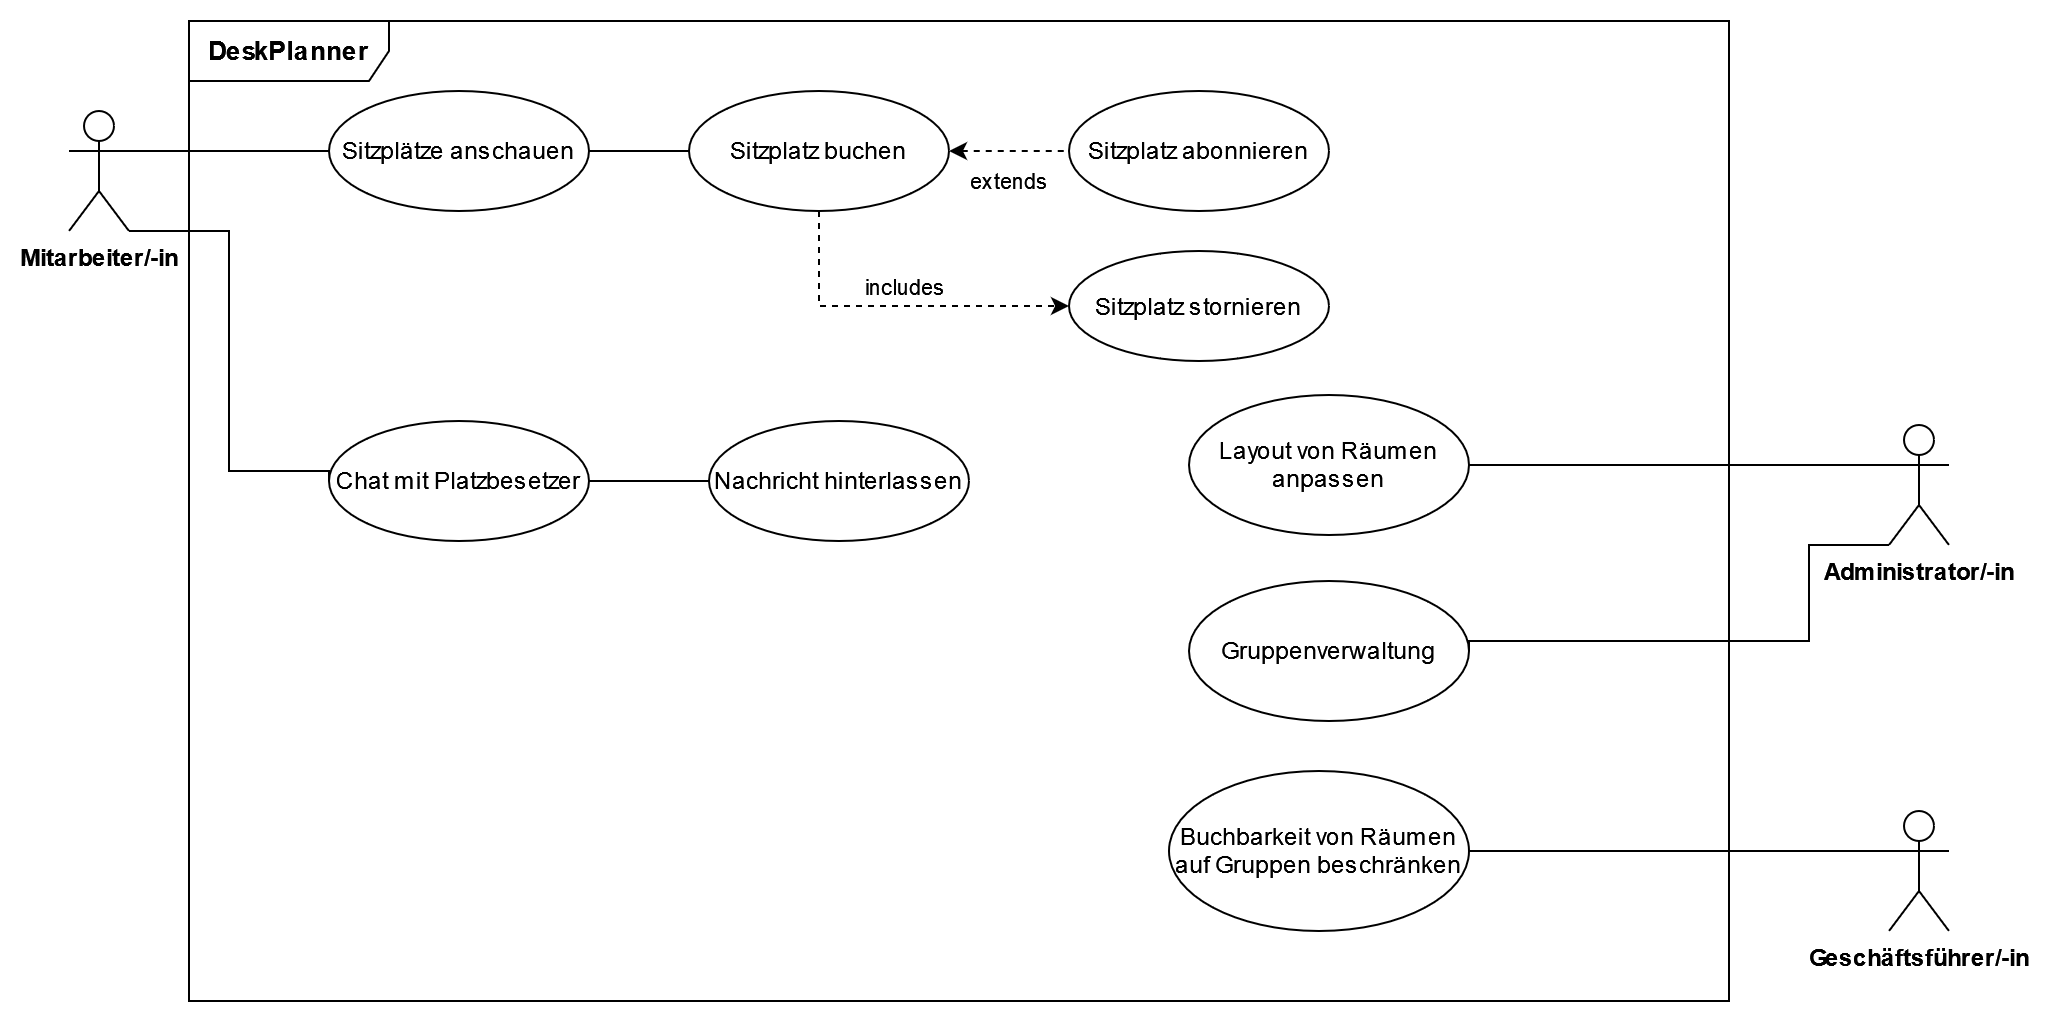
\includegraphics[width=0.8\textwidth]{UseCase_Diagram.png}
    \caption{Usecase-Diagramm}
    \label{fig:Usecase-Diagramm}
\end{figure}